\chapter{Risultati}
\label{sec:risultati}

Nel seguente capitolo verranno presentati i risultati ottenuti e le riflessioni maturate durante lo sviluppo del progetto. Le tematiche trattate durante l'analisi e la progettazione del marketplace sono state molteplici, tra queste la gestione delle \textit{Artist's Resale Right} \cite{resale-right}, equivalente del \textit{revenue share} è stata la più complessa. 

La gestione delle \textit{royalties} è un tema attualmente molto discusso. Non essendoci uno standard completo i principali marketplace decentralizzati hanno adottato delle soluzioni personali per la loro implementazione. Le problematiche che affliggono questo argomento sono principalmente due: l'interoperabilità tra più marketplace e il rafforzamento della distribuzione delle \textit{royalty}. Lo standard \textit{ERC2981} risolve unicamente la prima problematica rendendolo non attrattivo, dato che per un marketplace risulta essere più importante l'\textit{enforcement} del \textit{revenue share}. Nel caso in cui un marketplace non riuscisse a garantire il pagamento delle \textit{royalties} al creatore dell'asset, quest'ultimo non sarà incentivato ad utilizzare la piattaforma. Proprio per questo motivo, i marketplace decentralizzati hanno adottato soluzioni proprietarie per garantire l'\textit{enforcement} del \textit{revenue share}, ma non essendo interoperabili tra loro l'ecosistema decentralizzato risulta essere frammentato. In aggiunta, ottenere informazioni tecniche sulle soluzioni adottate è un processo arduo, il che può generare dei dubbi sulla loro effettiva affidabilità. Di seguito è presente la tabella \ref{table:implementazioni-royalty} che riassume le differenze sovracitate.


\begin{table}[H]
    \centering
    \renewcommand{\arraystretch}{1.5}
    \begin{adjustbox}{max width=1\textwidth}
        \begin{tabular}{| p{0.33\linewidth} | p{0.33\linewidth} | p{0.33\linewidth} |}
            \hline
            \rowcolor{mint-cream}
                                             & Interoperabilità                                                       & Enforcement                                      \\
            \hline
            Utilizzo di ERC2981             & Presente ma lo standard ERC2981 non è largamente utilizzato            & Se presente, unicamente sul marketplace in cui è stato creato l'asset \\
            \hline
            Soluzioni dei principali marketplace decentralizzati  & Spesso nessuna interoperabilità tra marketplace diversi & Asset scambiabile unicamente sul marketplace in cui è stato creato l'asset, quindi enforcement presente \\
            \hline
        \end{tabular}
    \end{adjustbox}
    \caption{Confronto implementazioni \textit{royalty}}
    \label{table:implementazioni-royalty}
\end{table}

Dal mio punto di vista, la soluzione migliore sarebbe avere uno standard completo che includa l'obbligo di pagamento e la distribuzione automatica delle \textit{royalties} non in maniera spontanea come avviene attualmente. Chiaramente la difficoltà tecnica risiede nell'impossibilità di modificare gli standard NFT già esistenti, ma essendo la tecnologia blockchain in uno stato di crescita e sviluppo, sarebbe riduttivo fermarsi e adattarsi per mantenere la compatibilità con gli attuali sistemi. Come descritto nel documento \textit{The Renaissance of Legacy Systems} \cite{warren2012renaissance} riguardante l'aggiornamento dei sistemi obsoleti, i tentativi di cambiamenti con le tecniche di manutenzione possono rivelarsi terribilmente costosi e non soddisfare i nuovi requisiti, poiché il sistema non è in grado di accogliere ulteriori funzionalità. In questo scenario, lo sforzo e i costi investiti nel sistema vanno sprecati. Sebbene le attuali soluzioni non siano perfette, sono comunque applicabili e adatte a dipendenza del contesto di utilizzo. Una tipologia di marketplace che potrebbe non necessitare di interoperabilità ma unicamente della certezza della suddivisione delle \textit{royalties} sono i marketplace proprietari, i quali vendono beni connessi ad un servizio da loro offerto. Questo genere di marketplace non è totalmente decentralizzato ma può beneficiare della sicurezza fornita dalla blockchain, nonché della garanzia di gestione delle \textit{royalties} concessa dagli smart contracts ma anche di ulteriori funzionalità personalizzate, come ad esempio il controllo sul prezzo di \textit{reselling}. Il mercato del gaming e dei ticket per eventi sono due esempi che potrebbero utilizzare un marketplace di questa tipologia. 


Analizzando più in dettaglio i marketplace di tipo decentralizzato, è possibile confermare che essi costituiscono enormi vantaggi in termine di sicurezza, privacy e trasparenza rispetto ai marketplace centralizzati. L'approccio verso la trasparenza è notabile all'interno della soluzione sviluppata, per esempio in figura \ref{fig:risultati_storico}, dove è visibile l'intero storico dell'asset, e in figura \ref{fig:risulati_royalty}, dove è possibile visualizzare la divisione delle \textit{royalties} all'acquisto di un asset.

\begin{figure}[H]
    \centering
    \fcolorbox{mint-cream}{white}{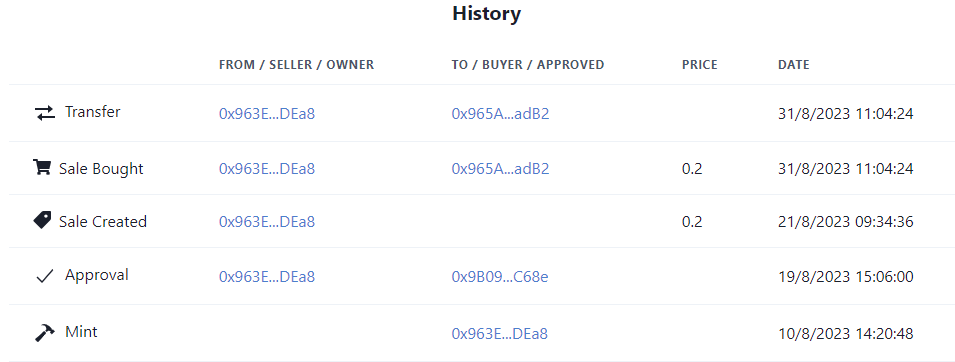
\includegraphics[width=\textwidth]{images/result_history.png}}
    \caption{Storico delle transazioni di un asset}
    \label{fig:risultati_storico}
\end{figure}

\begin{figure}[H]
    \centering
    \fcolorbox{mint-cream}{white}{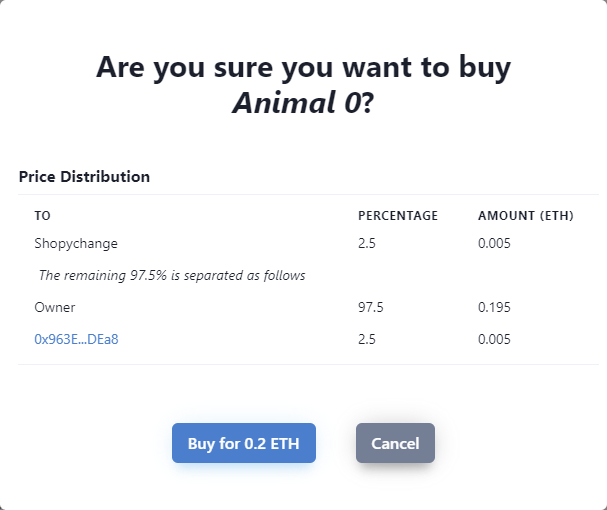
\includegraphics[width=0.6\textwidth]{images/result_royalty.png}}
    \caption{Divisione delle \textit{royalties} all'acquisto di un asset}  
    \label{fig:risulati_royalty}
\end{figure}

In aggiunta, sono in corso di sviluppo importanti funzionalità all'interno dei mercati decentralizzati, come ad esempio la possibilità di \textit{tokenizzare} beni fisici, come vestiti ed accessori, per poterli vendere in un ambiente decentralizzato. Ne è un esempio il progetto del famoso marchio \textit{Zara}, il quale ha lanciato una collezione di abiti \textit{NFT} che presentano la controparte fisica.  Questo concetto è estendibile ad un qualsiasi bene materiale, come ad esempio un'automobile o un immobile. \cite{belk2022money} Così facendo la società odierna risulterebbe essere più autonoma nelle transazioni commerciali, senza la necessità di intermediari ma con la possibilità di avere un ambiente sicuro e trasparente per portare a termine una trattativa. Il problema del concetto di \textit{tokenizzazione} risiede nell'effettivo trasferimento fisico del bene. 

Inoltre, in una situazione ipotetica potrebbe essere aggiunta la possibilità di frazionare la proprietà di un bene. Quest'ultima funzionalità risulterebbe utile nel concetto di \textit{revenue share}; il creatore possiederebbe una quota di proprietà, la quale aumenterebbe ad ogni rivendita, in modo da garantire un guadagno continuo in base al successo del bene. 

Tuttavia queste funzionalità sarebbero vane se non usufruite da un numero sufficiente di utenti. Personalmente trovo l'interfacciamento con la blockchain non adatto ad un utente medio, sarebbe necessaria una semplificazione dell'interazione con la blockchain per rendere la tecnologia più attrattiva agli utenti meno esperti. A tal proposito
sembrerebbe, infatti, che i \textit{GenZ} e i \textit{Millenials} (nati tra il 1980 e il 2012) siano più propensi alla detenzione di criptovalute rispetto alle generazioni precedenti. \cite{belk2022money}. Ciononostante sarebbe necessario un ulteriore studio per comprendere se questa tendenza è dovuta ad un interesse verso la tecnologia decentralizzata o semplicemente ad un fenomeno di \textit{FOMO} (\textit{Fear Of Missing Out}) a causa della forte volatilità del mercato. \cite{genz-fomo} 

Un altro aspetto da considerare è lo pseudonimato garantito dalla blockchain, il quale potrebbe portare ad un aumento di attività illecite.

\begin{figure}[H]
    \centering
    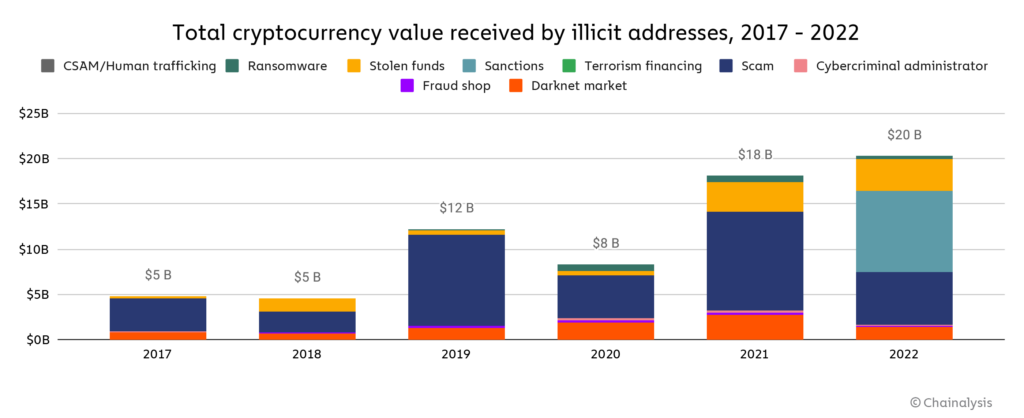
\includegraphics[width=\textwidth]{images/result_illecit.png}
    \caption{Attività illecite con criptovalute 2017 - 2022}  
    \label{fig:risultati_illecito}
\end{figure}

Come riportato dalle analisi di \textit{Chainalysis} \cite{chainalysis-money-laundering}, delle quali è possibile vedere un estratto in figura \ref{fig:risultati_illecito}, è stato riscontrato un incremento di attività illecite, in particolare di \textit{money laundering} attraverso l'uso delle principali criptovalute. Questo fenomeno è dovuto al fatto che, come spesso accade con tecnologie nuove, gli NFT offrono opportunità di abuso. Sebbene la tecnologia non è anonima ma pseudonima, ovvero non è possibile risalire all'identità di un utente ma è possibile ricostruire tutte le transazioni effettuate da un indirizzo, il che rappresenta comunque un problema per le autorità. \cite{bitstamp-privacy}

Concludendo, la tecnologia blockchain è uno strumento rivoluzionario che altererà il modo con il quale la società interagisce con i beni digitali e fisici. Tuttavia, sono necessari ulteriori sforzi implementativi e regolatori per rendere la tecnologia più accessibile e sicura.

% ***Problema***:
% - Eccessiva centralizzazione dei marketplace e troppa fiducia è riposta in essi


% ***Marketplace decentralizzato***: OK
% - Presenta degli enormi vantaggi rispetto a quello centralizzato. Es: sicurezza, privacy, controllo, censura, etc.


% - Gestione della tokenizzazione di un bene tangibile/fisico:
%  * https://www.vogue.com/article/zara-metaverse-collection, https://ww.fashionnetwork.com/news/Zara-returns-to-the-metaverse-with-zepeto,1515026.html


% - Money Laundering OK
%     *https://www.theverge.com/2022/2/2/22914056/nft-money-laundering-chainalysis
%     https://www.chainalysis.com/blog/2022-crypto-crime-report-preview-nft-wash-trading-money-laundering/


% - Troppo complesso per l'utente medio, usato da GenZ e Millenials OK
%     *https://dot.la/deloitte-gen-z-survey-2652644585.html
%     * https://www.fool.com/research/what-are-gen-z-millennial-investors-buying/
%     % * https://www.businessinsider.com/gen-z-are-investing-crypto-stocks-because-of-fomo-survey-2023-6?r=US&IR=T#:~:text=Redeem%20now-,Over%2040%25%20of%20Gen%20Z%20are%20investing%20because%20they're,and%20investing%20through%20social%20media.


% - La mancata regolarizzazione del mercato decentralizzato è un problema in quanto non si ha un controllo sulle transazioni e essendo anonime non si può risalire ai responsabili

